\documentclass[10pt]{article}
\author{Alex Peyrard}
\title{Digital Image Processing}
\usepackage{graphicx}

\begin{document}
\maketitle
\section{Introduction}
All of the programs are written in python 3. The shebangs are included and thus they should work if called using the "./program.py" notation. In case this causes a problem, please try to call them using "python3 program.py" notation.\\\\
I will provide further help on how to call each program.
\subsection{libraries}
I used numpy in all of the programs and scipy in some of them. I will detail when scipy is used.
\section{Exercise 1}
The program called ex1.py computes the histogram of a greyscale image, and enhances the image using histogram equalization. it displays the enhanced image, the histograms of the default and enhanced images, and the transformation function.\\
In this exercise, the matplotlib library is used to plot hitograms and functions.
\subsection{Examples}
\subsubsection{Fig1.jpg}
All of the results are obtained using the program with the call "./ex1.py Fig1.jpg"
\begin{figure}[!ht]
	\centering
	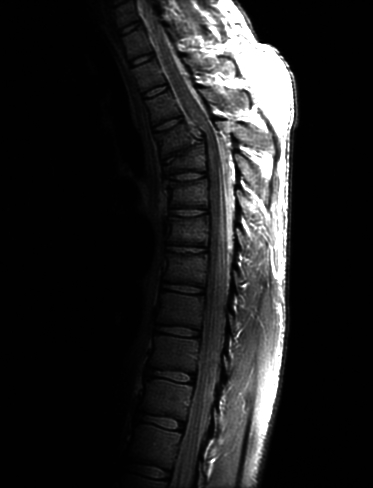
\includegraphics[height=200pt]{./ex1/Fig1.jpg}
	\caption{Original image}
\end{figure}
\begin{figure}[!ht]
	\centering
	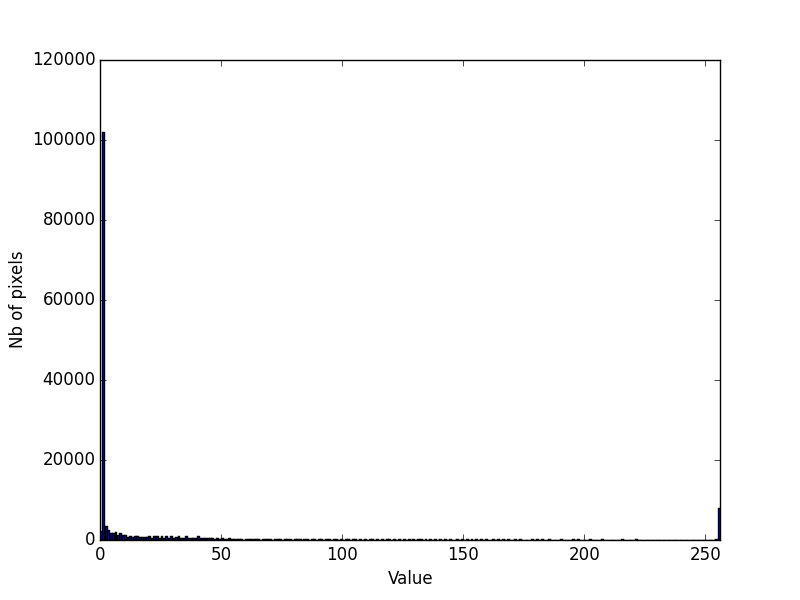
\includegraphics[height=200pt]{./ex1/Fig1_hist.png}
	\caption{Original image's histogram}
\end{figure}
\begin{figure}[!ht]
	\centering
	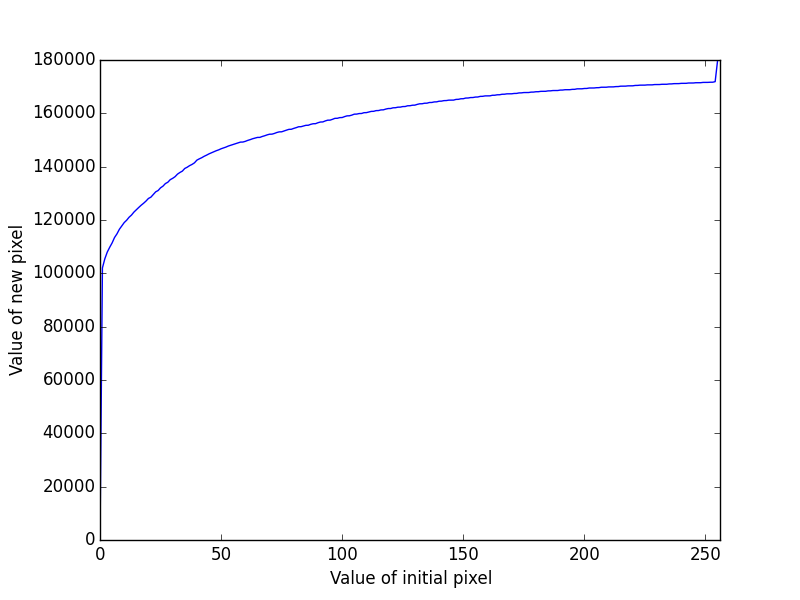
\includegraphics[height=200pt]{./ex1/Fig1_cdf.png}
	\caption{Enhancement function}
\end{figure}
\begin{figure}[!ht]
	\centering
	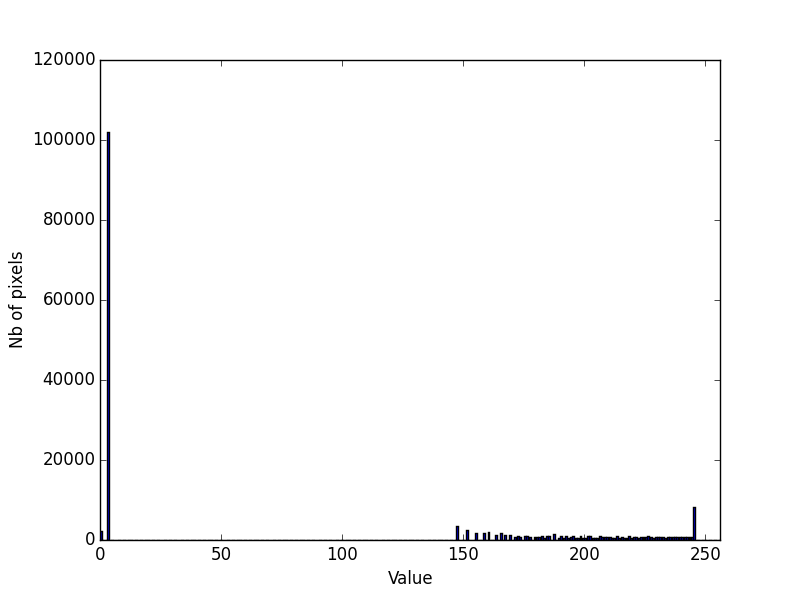
\includegraphics[height=200pt]{./ex1/Fig1_enh_hist.png}
	\caption{Enhanced image histogram}
\end{figure}
\begin{figure}[!ht]
	\centering
	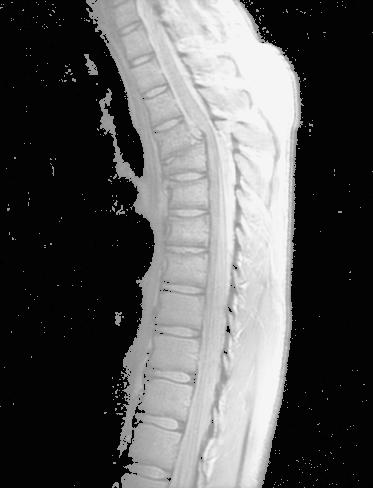
\includegraphics[height=200pt]{./ex1/Fig1_enh.jpg}
	\caption{Enhanced image}
\end{figure}
\clearpage

\subsubsection{Fig2.jpg}
All of the results are obtained using the program with the call "./ex1.py Fig2.jpg"
\begin{figure}[!ht]
	\centering
	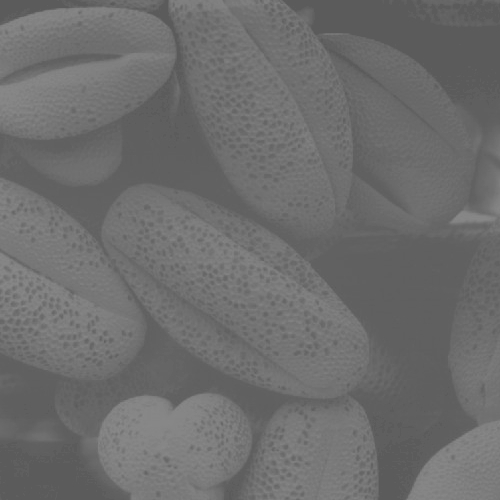
\includegraphics[height=200pt]{./ex1/Fig2.jpg}
	\caption{Original image}
\end{figure}
\begin{figure}[!ht]
	\centering
	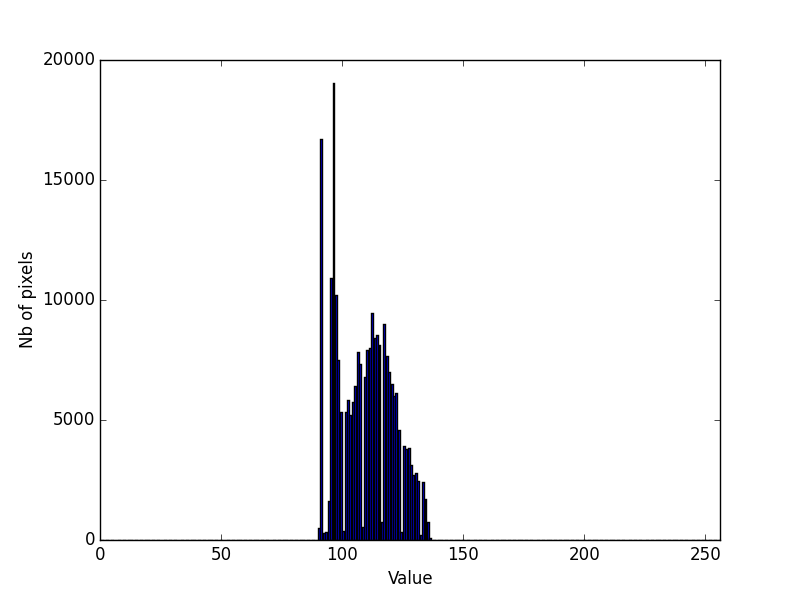
\includegraphics[height=200pt]{./ex1/Fig2_hist.png}
	\caption{Original image's histogram}
\end{figure}
\begin{figure}[!ht]
	\centering
	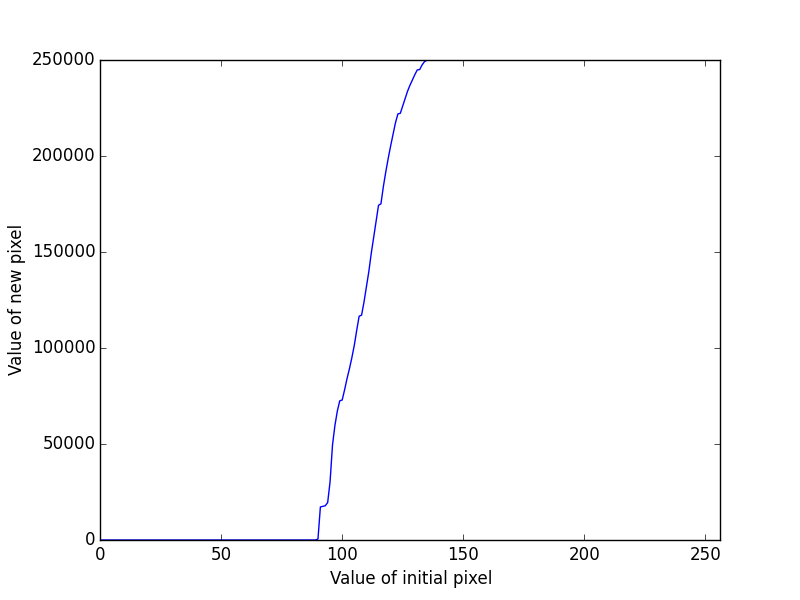
\includegraphics[height=200pt]{./ex1/Fig2_cdf.png}
	\caption{Enhancement function}
\end{figure}
\begin{figure}[!ht]
	\centering
	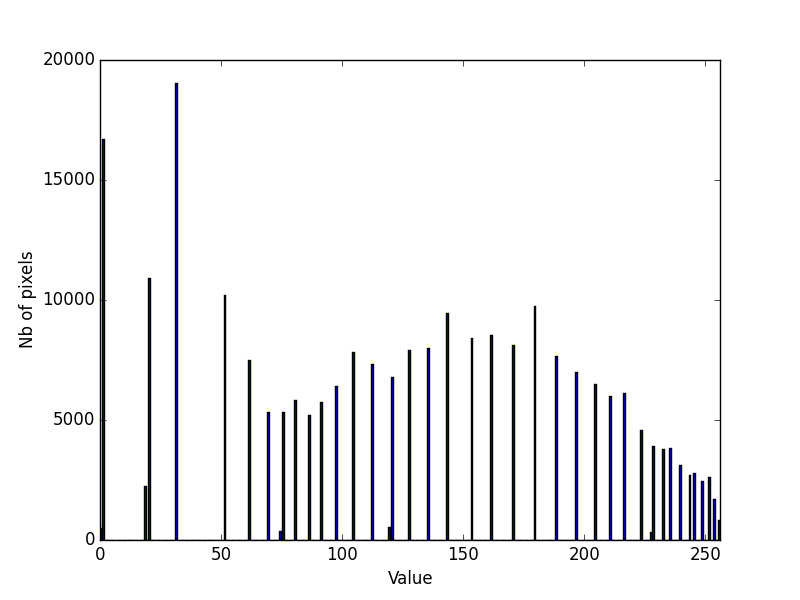
\includegraphics[height=200pt]{./ex1/Fig2_enh_hist.png}
	\caption{Enhanced image histogram}
\end{figure}
\begin{figure}[!ht]
	\centering
	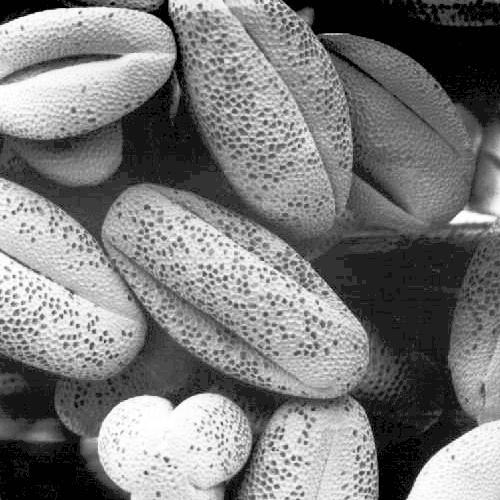
\includegraphics[height=200pt]{./ex1/Fig2_enh.jpg}
	\caption{Enhanced image}
\end{figure}
\clearpage

\section{Exercise 2}
The program called ex2.py performs several spatial enhancement techniques on a given greyscale image.
\subsection{Example on skeleton\_orig.tif}
All of the results are obtained using the program with the call "./ex2.py skeleton\_orig.tif"
\begin{figure}[!ht]
	\centering
	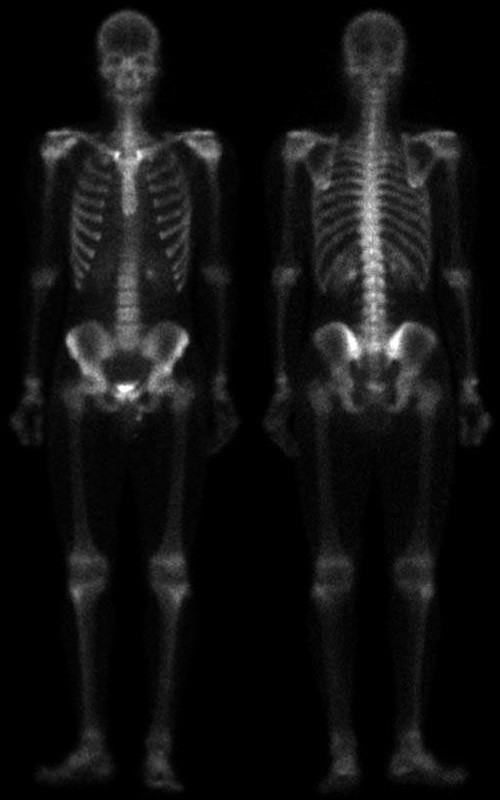
\includegraphics[height=200pt]{./ex2/skeleton_orig.jpg}
	\caption{Original image}
\end{figure}
\begin{figure}[!ht]
	\centering
	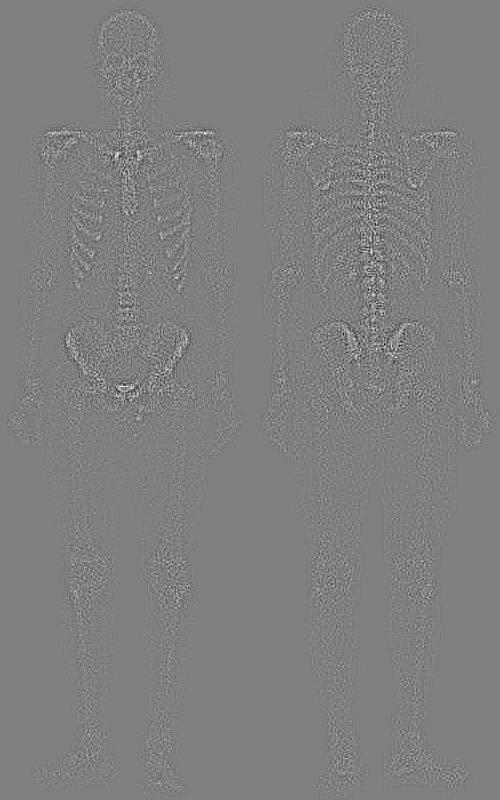
\includegraphics[height=200pt]{./ex2/skeleton_lap.jpg}
	\caption{Rescaled laplacian of image}
\end{figure}
\begin{figure}[!ht]
	\centering
	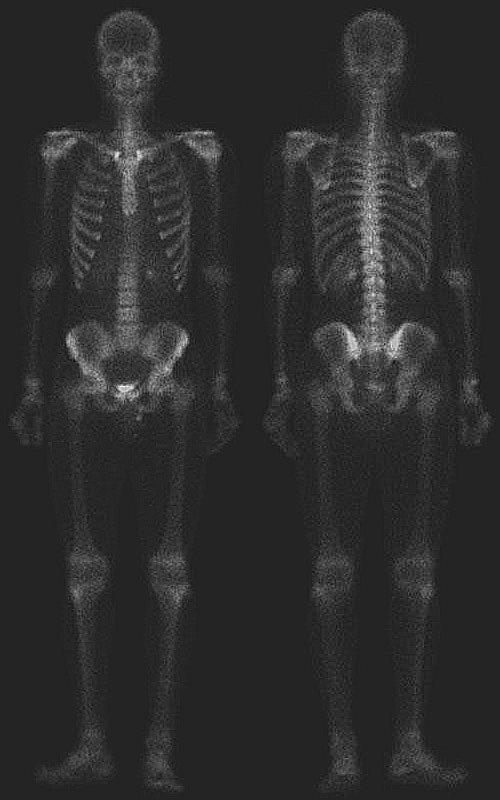
\includegraphics[height=200pt]{./ex2/skeleton_lap_plus_orig.jpg}
	\caption{Sum of laplacian and original image}
\end{figure}
\begin{figure}[!ht]
	\centering
	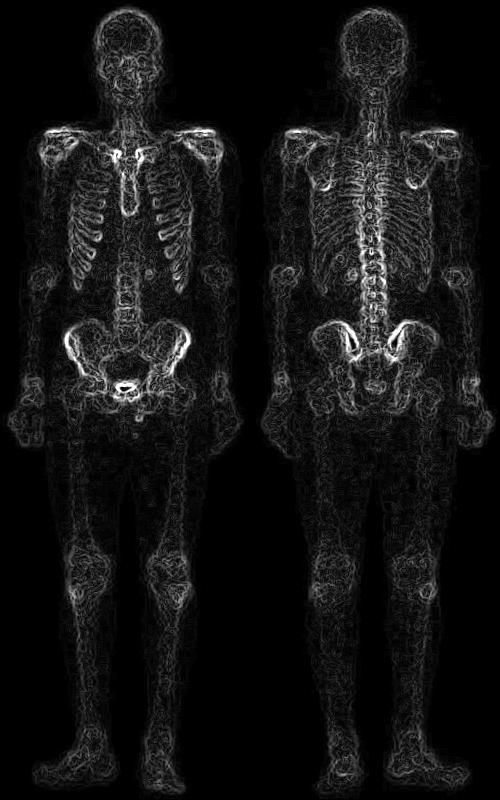
\includegraphics[height=200pt]{./ex2/skeleton_sobel.jpg}
	\caption{Sobel gradient of original image}
\end{figure}
\begin{figure}[!ht]
	\centering
	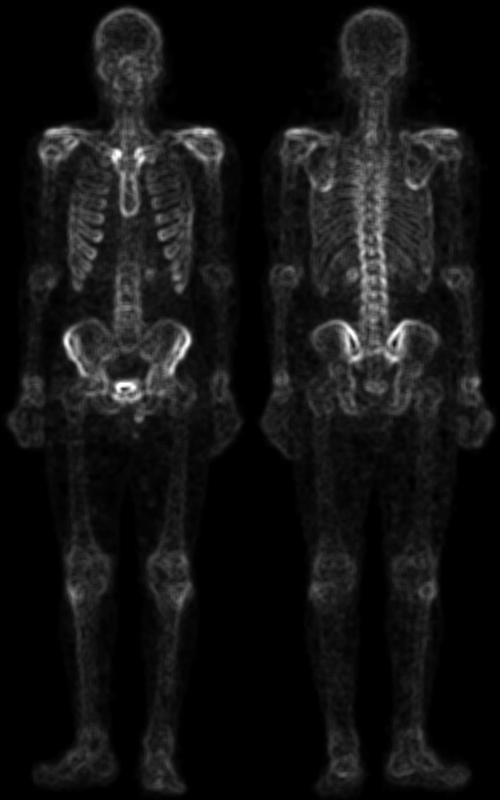
\includegraphics[height=200pt]{./ex2/skeleton_smmoth_sobel.jpg}
	\caption{Smoothed Sobel gradient of original image}
\end{figure}
\begin{figure}[!ht]
	\centering
	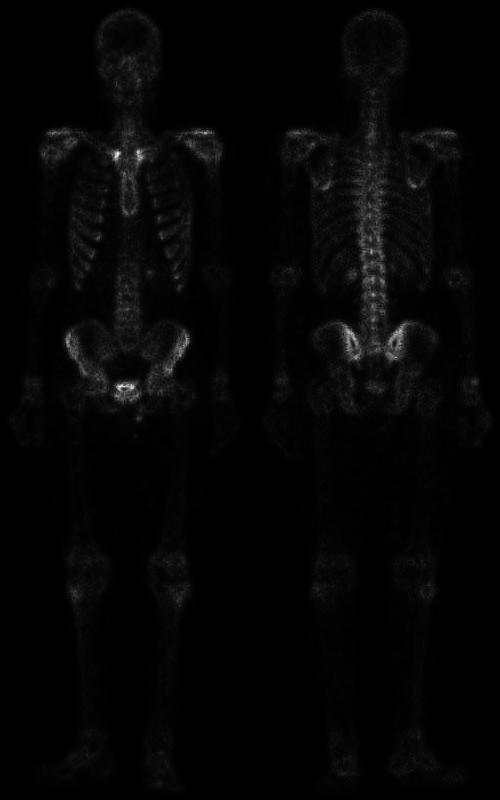
\includegraphics[height=200pt]{./ex2/skeleton_product.jpg}
	\caption{Product of smoothed Sobel gradient and of the previous sum of laplacian and original}
\end{figure}
\begin{figure}[!ht]
	\centering
	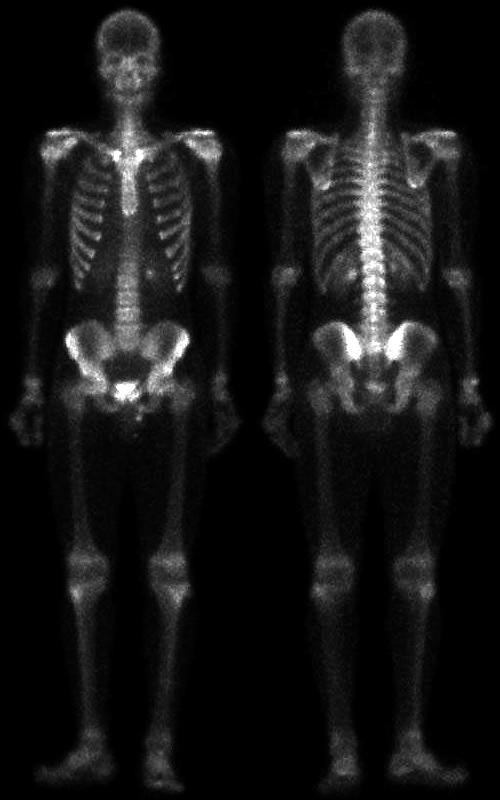
\includegraphics[height=200pt]{./ex2/skeleton_final.jpg}
	\caption{Sum of original image and previous image}
\end{figure}
\begin{figure}[!ht]
	\centering
	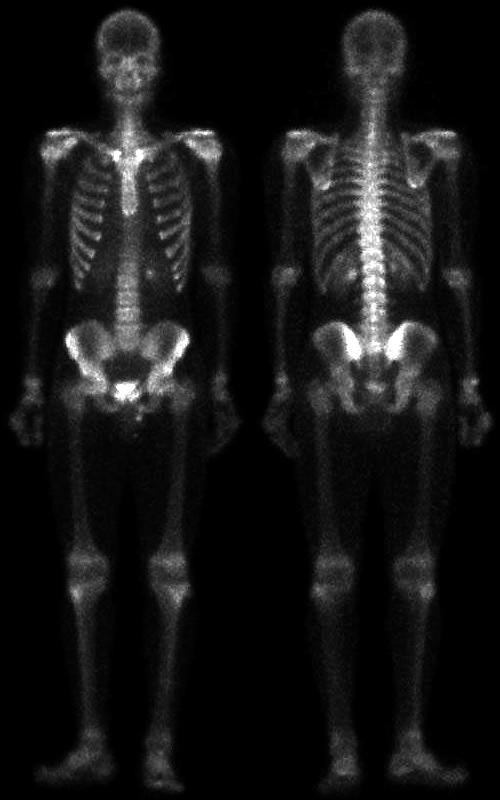
\includegraphics[height=200pt]{./ex2/skeleton_final.jpg}
	\caption{Power law of original image, gamma = 0.5, c = 1}
\end{figure}

\clearpage

\section{Exercise 3}
The program called ex3.py performs several frequency domain enhancement techniques on a given greyscale image.
\subsection{Examples}
\subsubsection{Ideal filter}
Those images are obtained using the call "./ex3 --ideal --highpass cutoff image" for highpass images, and "./ex3 --ideal --lowpass cutoff image" for lowpass images.
\begin{figure}[!ht]
	\centering
	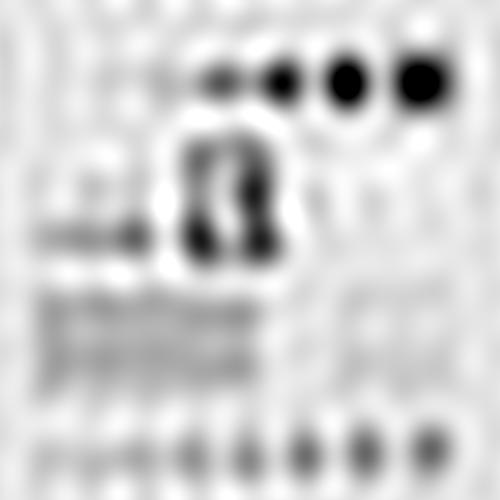
\includegraphics[height=200pt]{./ex3/ch_ideal_low_10.jpg}
	\caption{Cutoff 10 Ideal lowpass filter}
\end{figure}
\begin{figure}[!ht]
	\centering
	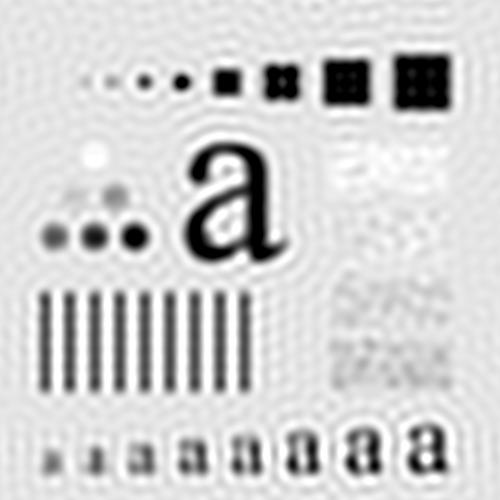
\includegraphics[height=200pt]{./ex3/ch_ideal_low_30.jpg}
	\caption{Cutoff 30 Ideal lowpass filter}
\end{figure}
\begin{figure}[!ht]
	\centering
	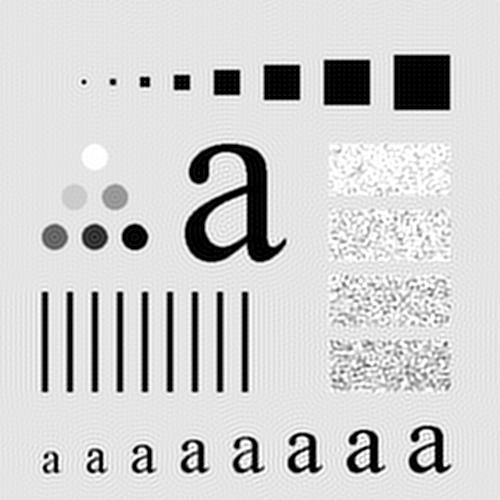
\includegraphics[height=200pt]{./ex3/ch_ideal_low_100.jpg}
	\caption{Cutoff 100 Ideal lowpass filter}
\end{figure}
\begin{figure}[!ht]
	\centering
	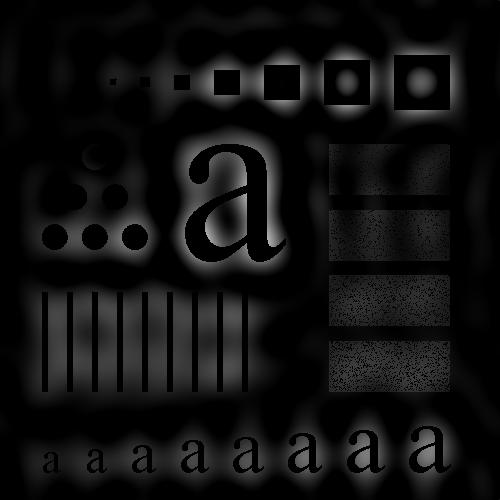
\includegraphics[height=200pt]{./ex3/ch_ideal_high_10.jpg}
	\caption{Cutoff 10 Ideal highpass filter}
\end{figure}
\begin{figure}[!ht]
	\centering
	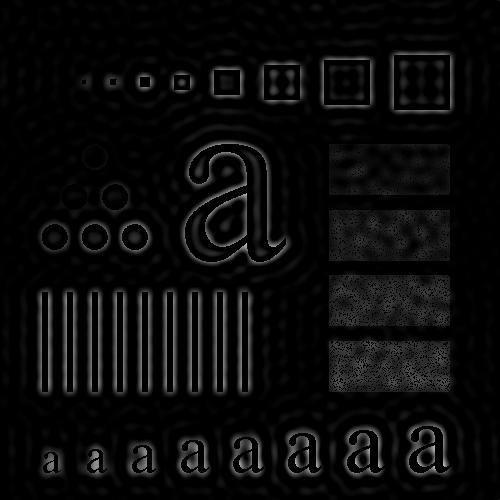
\includegraphics[height=200pt]{./ex3/ch_ideal_high_30.jpg}
	\caption{Cutoff 30 Ideal highpass filter}
\end{figure}
\begin{figure}[!ht]
	\centering
	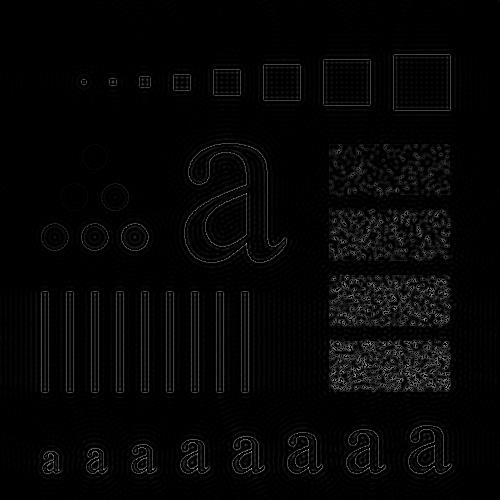
\includegraphics[height=200pt]{./ex3/ch_ideal_high_100.jpg}
	\caption{Cutoff 100 Ideal highpass filter}
\end{figure}
\clearpage
\subsubsection{Gaussian filter}
Those images are obtained using the call "./ex3 --gaussian --highpass cutoff image" for highpass images, and "./ex3 --gaussian --lowpass cutoff image" for lowpass images.
\begin{figure}[!ht]
	\centering
	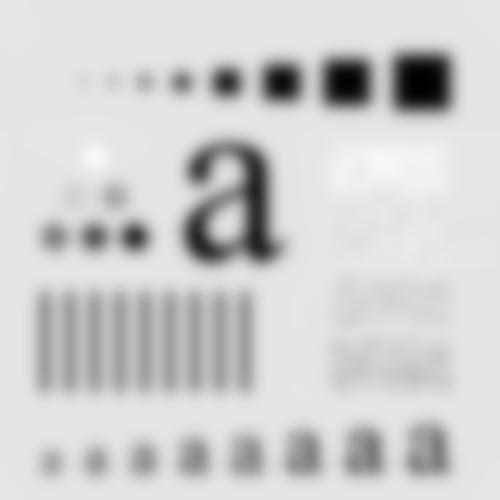
\includegraphics[height=200pt]{./ex3/ch_gauss_low_10.jpg}
	\caption{Cutoff 10 Gaussian lowpass filter}
\end{figure}
\begin{figure}[!ht]
	\centering
	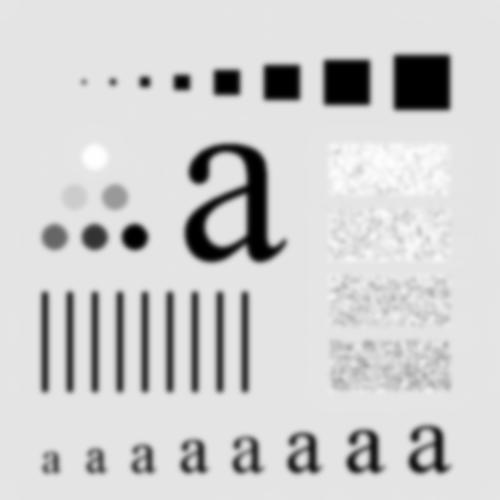
\includegraphics[height=200pt]{./ex3/ch_gauss_low_30.jpg}
	\caption{Cutoff 30 Gaussian lowpass filter}
\end{figure}
\begin{figure}[!ht]
	\centering
	
\includegraphics[height=200pt]{./ex3/ch_gauss_low_100.jpg}
	\caption{Cutoff 100 Gaussian lowpass filter}
\end{figure}
\begin{figure}[!ht]
	\centering
	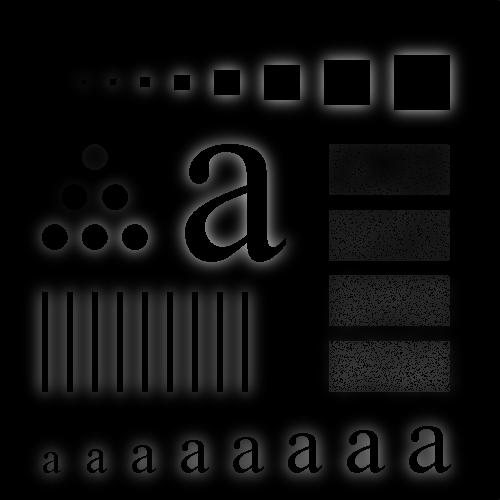
\includegraphics[height=200pt]{./ex3/ch_gauss_high_10.jpg}
	\caption{Cutoff 10 Gaussian highpass filter}
\end{figure}
\begin{figure}[!ht]
	\centering
	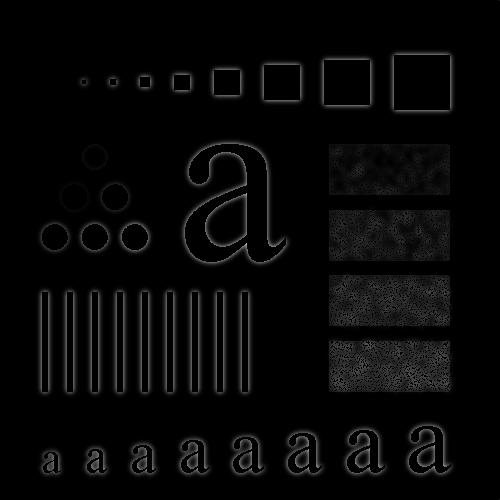
\includegraphics[height=200pt]{./ex3/ch_gauss_high_30.jpg}
	\caption{Cutoff 30 gaussian highpass filter}
\end{figure}
\begin{figure}[!ht]
	\centering
	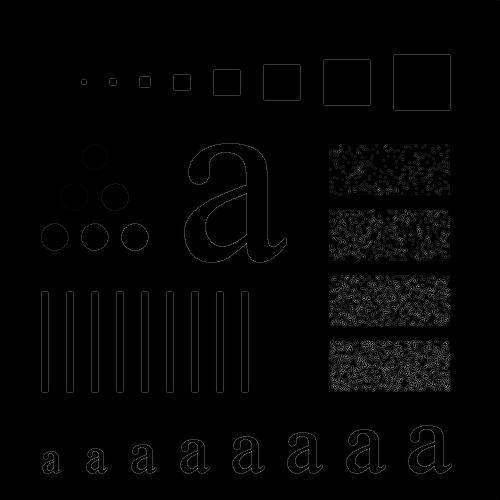
\includegraphics[height=200pt]{./ex3/ch_gauss_high_100.jpg}
	\caption{Cutoff 100 Gaussian highpass filter}
\end{figure}
\clearpage
\subsubsection{Butterworth filter}
Those images are obtained using the call "./ex3 --butterworth --highpass --order order cutoff image" for highpass images, and "./ex3 --butterworth --lowpass --order order cutoff image" for lowpass images.
\begin{figure}[!ht]
	\centering
	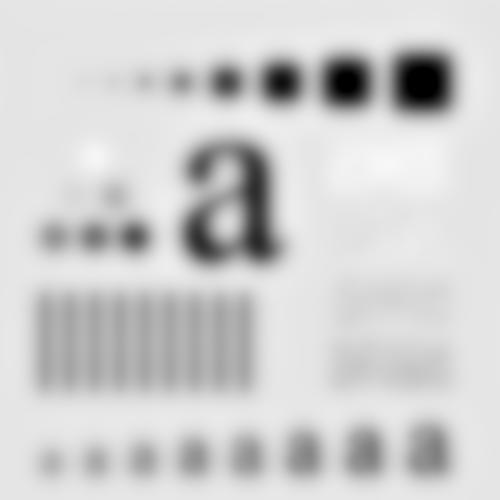
\includegraphics[height=200pt]{./ex3/ch_butter_low_10.jpg}
	\caption{Cutoff 10 order 2 Butterworth lowpass filter}
\end{figure}
\begin{figure}[!ht]
	\centering
	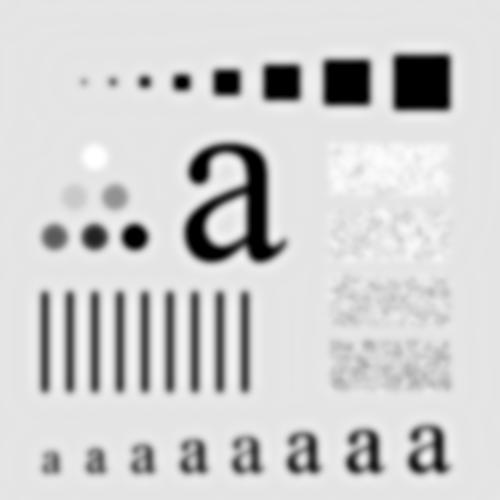
\includegraphics[height=200pt]{./ex3/ch_butter_low_30.jpg}
	\caption{Cutoff 30 order 2 Butterworth lowpass filter}
\end{figure}

\begin{figure}[!ht]
	\centering
	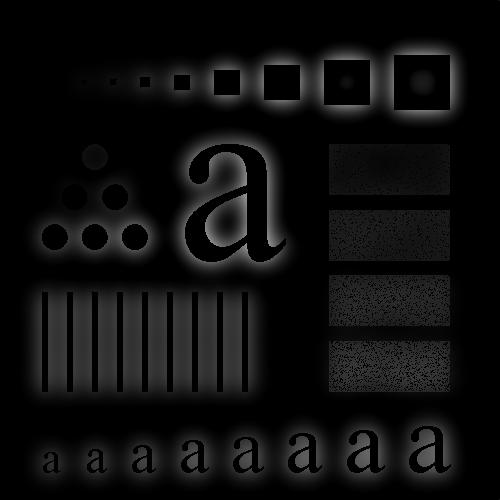
\includegraphics[height=200pt]{./ex3/ch_butter_high_10.jpg}
	\caption{Cutoff 10 order 2 Butterworth highpass filter}
\end{figure}
\begin{figure}[!ht]
	\centering
	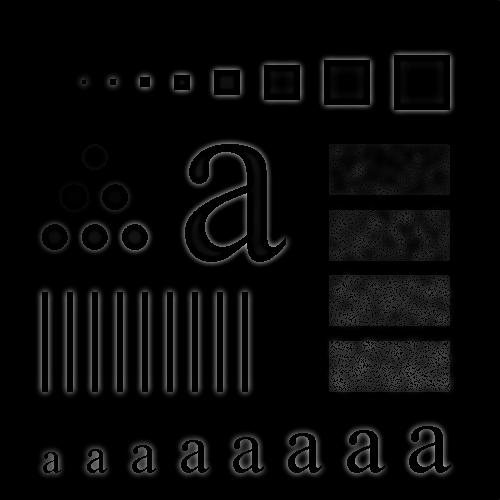
\includegraphics[height=200pt]{./ex3/ch_butter_high_30.jpg}
	\caption{Cutoff 30 order 2 Butterworth highpass filter}
\end{figure}

\clearpage

\section{Exercise 4}
For exercise 4, the program gaussNoise.py adds gaussian noise of desired mean and variance o an image.
The program uniNoise.py adds uniform noise of desired lower and upper bound to an image.
The program filtering.py uses different means of filtering an image.
\subsection{Examples}
\begin{figure}[!ht]
	\centering
	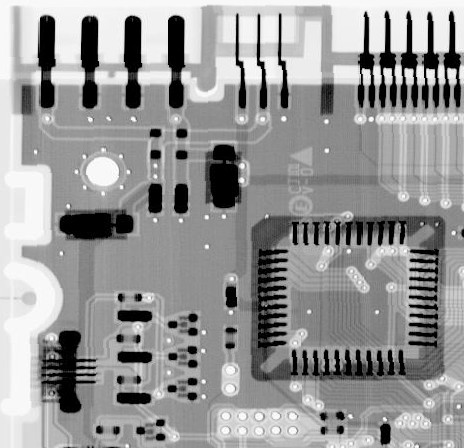
\includegraphics[height=200pt]{./ex4/Circuit.jpg}
	\caption{Original image}
\end{figure}
\begin{figure}[!ht]
	\centering
	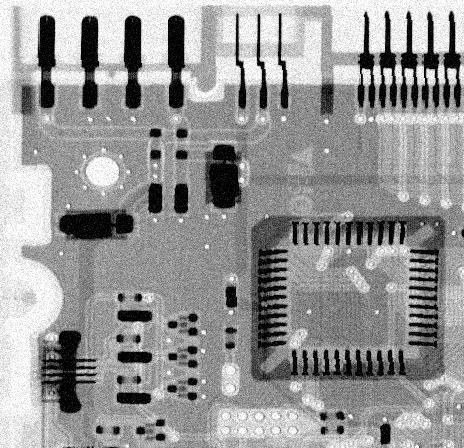
\includegraphics[height=200pt]{./ex4/gaussC.jpg}
	\caption{Original image with gaussian noise of mean 0 and variance 260}
\end{figure}
\begin{figure}[!ht]
	\centering
	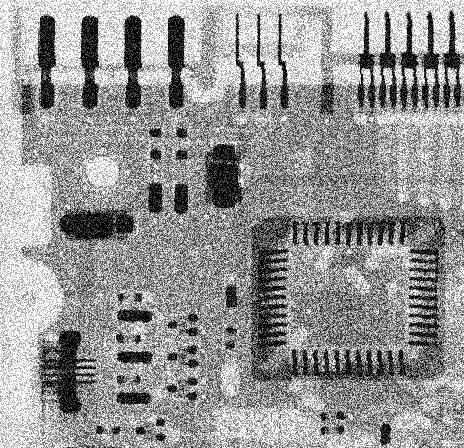
\includegraphics[height=200pt]{./ex4/uniC.jpg}
	\caption{Original image with uniform noise in the [-100, 100] range}
\end{figure}
\begin{figure}[!ht]
	\centering
	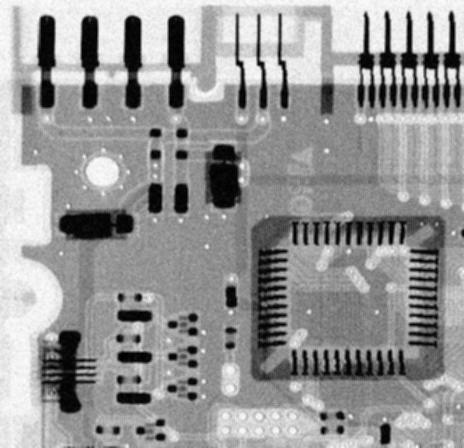
\includegraphics[height=200pt]{./ex4/gaussarith.jpg}
	\caption{Image with gaussian noise enhanced with arithmetic mean}
\end{figure}
\begin{figure}[!ht]
	\centering
	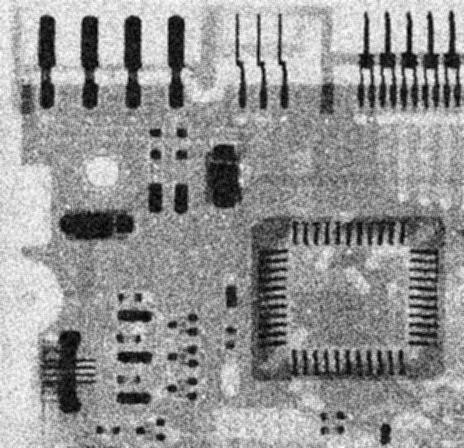
\includegraphics[height=200pt]{./ex4/uniarith.jpg}
	\caption{Image with uniform noise enhanced with arithmetic mean}
\end{figure}

\begin{figure}[!ht]
	\centering
	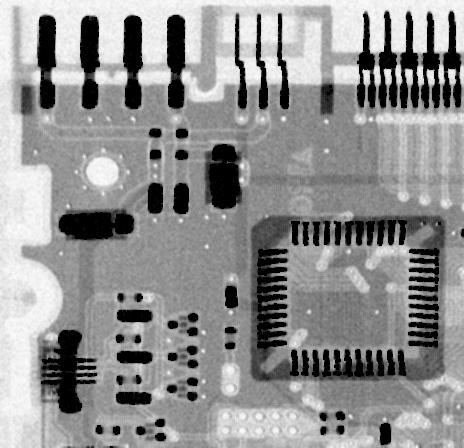
\includegraphics[height=200pt]{./ex4/gaussgeo.jpg}
	\caption{Image with gaussian noise enhanced with geometric mean}
\end{figure}
\begin{figure}[!ht]
	\centering
	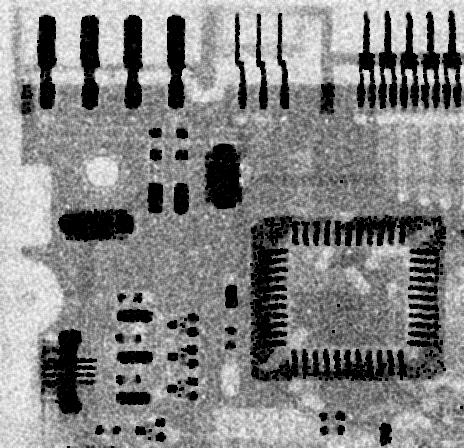
\includegraphics[height=200pt]{./ex4/unigeo.jpg}
	\caption{Image with uniform noise enhanced with geometric mean}
\end{figure}

\begin{figure}[!ht]
	\centering
	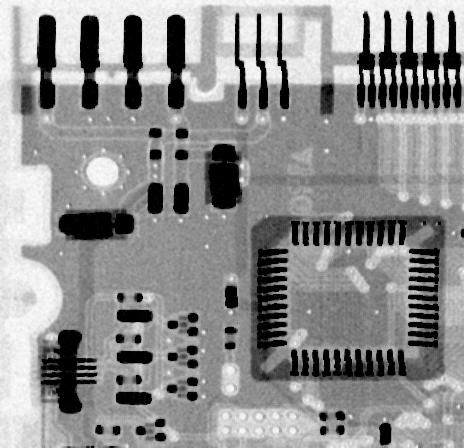
\includegraphics[height=200pt]{./ex4/gaussharmo.jpg}
	\caption{Image with gaussian noise enhanced with harmonic filter}
\end{figure}
\begin{figure}[!ht]
	\centering
	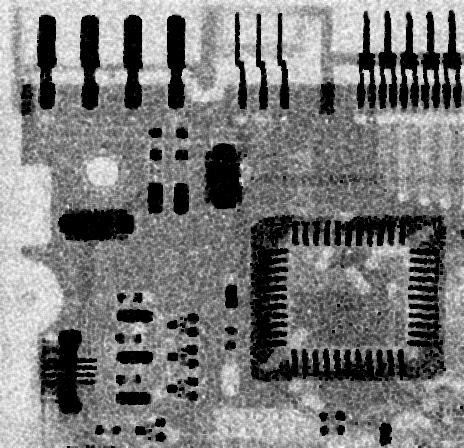
\includegraphics[height=200pt]{./ex4/uniharmo.jpg}
	\caption{Image with uniform noise enhanced with harmonic filter}
\end{figure}

\begin{figure}[!ht]
	\centering
	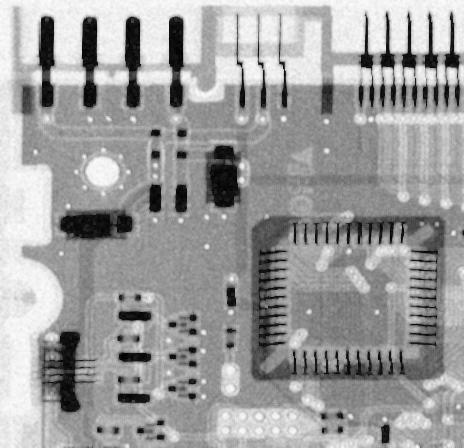
\includegraphics[height=200pt]{./ex4/gaussch15.jpg}
	\caption{Image with gaussian noise enhanced with contra harmonic filter of order 1.5}
\end{figure}
\begin{figure}[!ht]
	\centering
	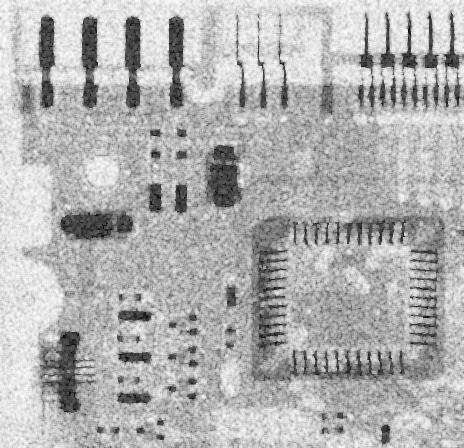
\includegraphics[height=200pt]{./ex4/unich15.jpg}
	\caption{Image with uniform noise enhanced with contra harmonic filter of order 1.5}
\end{figure}

\begin{figure}[!ht]
	\centering
	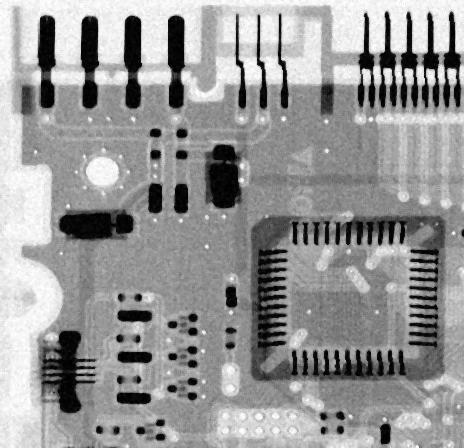
\includegraphics[height=200pt]{./ex4/gaussmedian.jpg}
	\caption{Image with gaussian noise enhanced with median filter}
\end{figure}
\begin{figure}[!ht]
	\centering
	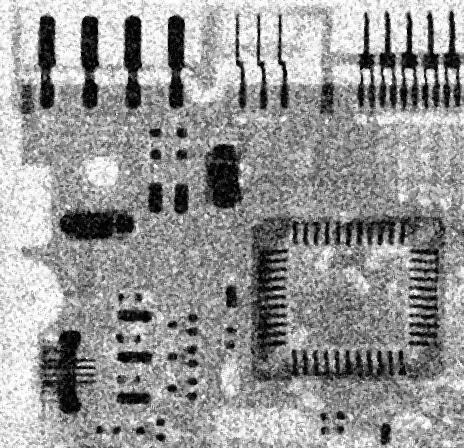
\includegraphics[height=200pt]{./ex4/unimedian.jpg}
	\caption{Image with uniform noise enhanced with median filter}
\end{figure}

\begin{figure}[!ht]
	\centering
	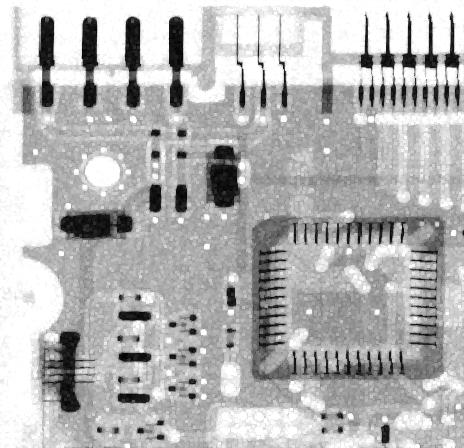
\includegraphics[height=200pt]{./ex4/gaussmax.jpg}
	\caption{Image with gaussian noise enhanced with max filter}
\end{figure}
\begin{figure}[!ht]
	\centering
	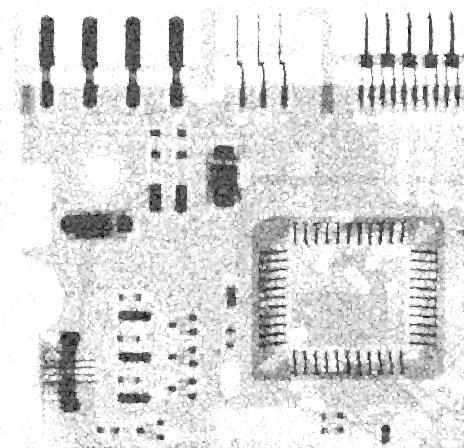
\includegraphics[height=200pt]{./ex4/unimax.jpg}
	\caption{Image with uniform noise enhanced with max filter}
\end{figure}

\begin{figure}[!ht]
	\centering
	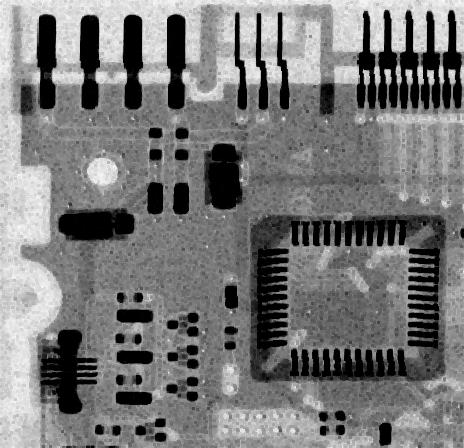
\includegraphics[height=200pt]{./ex4/gaussmin.jpg}
	\caption{Image with gaussian noise enhanced with min filter}
\end{figure}
\begin{figure}[!ht]
	\centering
	\includegraphics[height=200pt]{./ex4/unimin.jpg}
	\caption{Image with uniform noise enhanced with min filter}
\end{figure}

\clearpage
\begin{figure}[!ht]
	\centering
	\includegraphics[height=200pt]{./ex4/gaussmid.jpg}
	\caption{Image with gaussian noise enhanced with midpoint filter}
\end{figure}
\begin{figure}[!ht]
	\centering
	\includegraphics[height=200pt]{./ex4/unimid.jpg}
	\caption{Image with uniform noise enhanced with midpoint filter}
\end{figure}

\begin{figure}[!ht]
	\centering
	\includegraphics[height=200pt]{./ex4/gaussalpha2.jpg}
	\caption{Image with gaussian noise enhanced with alpha trimmed filter of order 2}
\end{figure}
\begin{figure}[!ht]
	\centering
	\includegraphics[height=200pt]{./ex4/unialpha2.jpg}
	\caption{Image with uniform noise enhanced with alpha trimmed filter of order 2}
\end{figure}


\clearpage
\section{Exercice 5}
In exercise 5 we analyze blurring degradation.\\
Using "./ex5 blur image output" The program blurs and saves an image.\\
By using "./ex5 filter image output", the program enhances a blurred image using the inverse filter.
\section{Example}
\begin{figure}[!ht]
	\centering
	\includegraphics[height=200pt]{./ex5/book_cover.jpg}
	\caption{Original image}
\end{figure}
\begin{figure}[!ht]
	\centering
	\includegraphics[height=200pt]{./ex5/blurredBook.jpg}
	\caption{Blurred image}
\end{figure}
\begin{figure}[!ht]
	\centering
	\includegraphics[height=200pt]{./ex5/blurredGaussBook.jpg}
	\caption{Blurred image with gaussian noise of mean 0 variance 650}
\end{figure}
\begin{figure}[!ht]
	\centering
	\includegraphics[height=200pt]{./ex5/filteredBook.jpg}
	\caption{Enhanced image of the blurred book}
\end{figure}
\begin{figure}[!ht]
	\centering
	\includegraphics[height=200pt]{./ex5/filteredGaussBook.jpg}
	\caption{Enhanced image of the blurred book with noise}
\end{figure}
\clearpage

We can notice that the enhancement with inverse filtering isn't perfect, and is useless with noise.\\

I apologize for not being able to do the rest of the exercise.

\section{Exercise 6}
This program is capable of performing rotations, translations and rescaling on an image, using either the nearest neighbor or bilinear interpolation.\\

Usage :\\
--neighbor for nearest neighbor\\
--bilinear for bilinear interpolation\\

--rotate, --rescale, --translate to choose transform
\subsection{Examples}
\begin{figure}[!ht]
	\centering
	\includegraphics[height=200pt]{./ex6/ray_trace_bottle.jpg}
	\caption{Original image}
\end{figure}
\begin{figure}[!ht]
	\centering
	\includegraphics[height=200pt]{./ex6/rotate26n.jpg}
	\caption{Image rotated by 26 degrees with nearest neighbor. Command line : ./ex6 --neighbor --rotate image 26}
\end{figure}
\begin{figure}[!ht]
	\centering
	\includegraphics[height=200pt]{./ex6/rotate155b.jpg}
	\caption{Image rotated by 155 degrees with bilinear interpolation. Command line : ./ex6 --bilinear --rotate image 155}
\end{figure}
\begin{figure}[!ht]
	\centering
	\includegraphics[height=200pt]{./ex6/rescale05.jpg}
	\caption{Image rescaled by 0.5 with nearest neighbor. Command line : ./ex6 --neighbor --rescale image 0.5}
\end{figure}
\begin{figure}[!ht]
	\centering
	\includegraphics[height=200pt]{./ex6/rescale2.jpg}
	\caption{Image rescaled by 2 with bilinear interpolation. Command line : ./ex6 --bilinear --rescale image 2}
\end{figure}
\begin{figure}[!ht]
	\centering
	\includegraphics[height=200pt]{./ex6/translate1.jpg}
	\caption{Image translated by 166.5 -455.3 with nearest neighbor. Command line : ./ex6 --neighbor --translate image 166.5 -455.3}
\end{figure}
\begin{figure}[!ht]
	\centering
	\includegraphics[height=200pt]{./ex6/translate2.jpg}
	\caption{Image translated by -25.12 65 with bilinear interpolation. Command line : ./ex6 --bilinear --translate image -25.12 65}
\end{figure}
\clearpage
\section{Exercise 7}
The exercise 7 program can compress an image using the discrete cosine transform and a mask to discard coefficients.\\

Usage :\\
--dct to perform the dct\\
--showdiff to show the differences between the original image and the compressed image\\

--threshold to use the threshold mask instead of the zonal mask.
\subsection{Examples}
\begin{figure}[!ht]
	\centering
	\includegraphics[height=200pt]{./ex7/lenna.jpg}
	\caption{Original image}
\end{figure}
\begin{figure}[!ht]
	\centering
	\includegraphics[height=200pt]{./ex7/zonal.jpg}
	\caption{Image compressed using the zonal mask}
\end{figure}
\clearpage
\begin{figure}[!ht]
	\centering
	\includegraphics[height=200pt]{./ex7/zonaldiff.jpg}
	\caption{Differences between original and zonal compressed images}
\end{figure}

\begin{figure}[!ht]
	\centering
	\includegraphics[height=200pt]{./ex7/threshold.jpg}
	\caption{Image compressed using the zonal mask}
\end{figure}
\begin{figure}[!ht]
	\centering
	\includegraphics[height=200pt]{./ex7/thresholddiff.jpg}
	\caption{Differences between original and zonal compressed images}
\end{figure}

\clearpage

I wasn't able to do the part of the exercise with wavelets.

\section{Exercise 8}
The exercise 8 program can perform morphological processing on an image.\\

Usage :\\ 
--dilate to use dilation\\
--erode to use erosion\\
--open to use opening\\
--close to use closing\\

--boundary to use boundary extraction\\
--filling to use hole filling\\
--extraction for feature extraction

\subsection{Examples}
\begin{figure}[!ht]
	\centering
	\includegraphics[height=200pt]{./ex8/noisy_fingerprint.jpg}
	\caption{Original image}
\end{figure}
\begin{figure}[!ht]
	\centering
	\includegraphics[height=200pt]{./ex8/noisy_dilated.jpg}
	\caption{Dilated image. Command ./ex8 --dilate image}
\end{figure}
\begin{figure}[!ht]
	\centering
	\includegraphics[height=200pt]{./ex8/noisy_eroded.jpg}
	\caption{Eroded image. Command ./ex8 --erode image}
\end{figure}
\begin{figure}[!ht]
	\centering
	\includegraphics[height=200pt]{./ex8/noisy_opened.jpg}
	\caption{Opened image. Command ./ex8 --open image}
\end{figure}
\begin{figure}[!ht]
	\centering
	\includegraphics[height=200pt]{./ex8/noisy_closed.jpg}
	\caption{Closed image. Command ./ex8 --close image}
\end{figure}
\begin{figure}[!ht]
	\centering
	\includegraphics[height=200pt]{./ex8/lincoln.jpg}
	\caption{Original image}
\end{figure}
\begin{figure}[!ht]
	\centering
	\includegraphics[height=200pt]{./ex8/lincoln_boundary.jpg}
	\caption{Boundary of image. Command ./ex8 --boundary image}
\end{figure}
\begin{figure}[!ht]
	\centering
	\includegraphics[height=200pt]{./ex8/region.jpg}
	\caption{Original image}
\end{figure}
\begin{figure}[!ht]
	\centering
	\includegraphics[height=200pt]{./ex8/region_filled.jpg}
	\caption{Image filled at position 50 50. Command ./ex8 --filling image 50 50}
\end{figure}

\begin{figure}[!ht]
	\centering
	\includegraphics[height=150pt]{./ex8/chicken.jpg}
	\caption{Original image}
\end{figure}
\begin{figure}[!ht]
	\centering
	\includegraphics[height=150pt]{./ex8/chicken_extracted.jpg}
	\caption{Image thresholded, eroded, and then extracted at position 100 356. Command ./ex8 --extraction image 100 356}
\end{figure}
\clearpage
The program also gives the number of pixels of the extracted component. In this case :  1356 pixels
\clearpage
\section{Exercise 9}
The exercise 9 program can perform image segmentation on an image using edge detectors or thresholding segmentation methods.\\

Usage : \\
--roberts to use the Roberts edge detectors\\
--prewitt to use the Prewitt edge detector\\
--sobel to use the Sobel edge detector\\
--mh to use the Marr hildreth edge detector\\
--canny to use the canny edge detector\\

--otsu to use Otsu's threshold segmentation.\\
--threshold to use the global thresholding method
\subsection{Examples}
\begin{figure}[!ht]
	\centering
	\includegraphics[height=200pt]{./ex9/building.jpg}
	\caption{Original image}
\end{figure}
\begin{figure}[!ht]
	\centering
	\includegraphics[height=200pt]{./ex9/building_roberts.jpg}
	\caption{Image obtained using Roberts edge detector. Command : ./ex9 --roberts image}
\end{figure}
\begin{figure}[!ht]
	\centering
	\includegraphics[height=200pt]{./ex9/building_prewitt.jpg}
	\caption{Image obtained using Prewitt edge detector. Command : ./ex9 --prewitt image}
\end{figure}
\begin{figure}[!ht]
	\centering
	\includegraphics[height=200pt]{./ex9/building_sobel.jpg}
	\caption{Image obtained using Sobel edge detector. Command : ./ex9 --sobel image}
\end{figure}
\begin{figure}[!ht]
	\centering
	\includegraphics[height=200pt]{./ex9/building_mh.jpg}
	\caption{Image obtained using Marr Hildreth edge detector. Command : ./ex9 --mh image}
\end{figure}
\begin{figure}[!ht]
	\centering
	\includegraphics[height=200pt]{./ex9/building_canny.jpg}
	\caption{Image obtained using Canny edge detector. Command : ./ex9 --canny image}
\end{figure}
\begin{figure}[!ht]
	\centering
	\includegraphics[height=200pt]{./ex9/polymersomes.jpg}
	\caption{Original image}
\end{figure}
\begin{figure}[!ht]
	\centering
	\includegraphics[height=200pt]{./ex9/polymersomes_otsu.jpg}
	\caption{Image obtained using Otsu's method. Command : ./ex9 --otsu image. Obtained $\eta$ : 0.48}
\end{figure}
\begin{figure}[!ht]
	\centering
	\includegraphics[height=200pt]{./ex9/polymersomes_global.jpg}
	\caption{Image obtained using global thresholding method method. Command : ./ex9 --threshold image.}
\end{figure}
\clearpage
We can see that Otsu's method is better at determining the best threshold value./
\section{Exercise 10}
The exercise 10 program can perform boundary following, resampling, and compute the chain code and the difference chain code of a grayscale image.\\

The pca program can use principal component analysis to compress an image and reconstruct it from fewer components.

Usage of ex10: \\
--boundary to use boundary following\\
--resampling to use boundary following and resampling\\
--linking to link the resampled points\\
--chain to compute the chain code\\
--chaindiff to compute the difference chain code\\

Usage of pca:
calling pca automatically reconstructs the 6 images from washington DC from 2 components and also prints the difference images.
\subsection{Examples}
\begin{figure}[!ht]
	\centering
	\includegraphics[height=200pt]{./ex10/noisy_stroke.jpg}
	\caption{Original image}
\end{figure}
\begin{figure}[!ht]
	\centering
	\includegraphics[height=200pt]{./ex10/noisy_boundary.jpg}
	\caption{Boundary of the image. Command : ./ex10 --boundary image}
\end{figure}
\begin{figure}[!ht]
	\centering
	\includegraphics[height=200pt]{./ex10/noisy_resample.jpg}
	\caption{Resampling of the image's boundary. Command : ./ex10 --resampling image}
\end{figure}
\begin{figure}[!ht]
	\centering
	\includegraphics[height=200pt]{./ex10/noisy_link.jpg}
	\caption{Linking of the previous image. Command : ./ex10 --linking image}
\end{figure}
\clearpage
The chain code, obtained with ./ex10 --chain image, is 0000606666666646442444242222202202\\

The first difference chain code, obtained with ./ex10 --chaindiff image, is 
000626000000062606200626000062062\\

Images used for pca :
\begin{figure}[!ht]
	\centering
	\includegraphics[height=200pt]{./ex10/WashingtonDC_Band1.jpg}
	\caption{Original image 1}
\end{figure}
\begin{figure}[!ht]
	\centering
	\includegraphics[height=200pt]{./ex10/WashingtonDC_Band2.jpg}
	\caption{Original image 2}
\end{figure}
\begin{figure}[!ht]
	\centering
	\includegraphics[height=200pt]{./ex10/WashingtonDC_Band3.jpg}
	\caption{Original image 3}
\end{figure}
\begin{figure}[!ht]
	\centering
	\includegraphics[height=200pt]{./ex10/WashingtonDC_Band4.jpg}
	\caption{Original image 4}
\end{figure}
\begin{figure}[!ht]
	\centering
	\includegraphics[height=200pt]{./ex10/WashingtonDC_Band5.jpg}
	\caption{Original image 5}
\end{figure}
\begin{figure}[!ht]
	\centering
	\includegraphics[height=200pt]{./ex10/WashingtonDC_Band6.jpg}
	\caption{Original image 6}
\end{figure}
\clearpage
Images obtained with 2 remaining components :
\begin{figure}[!ht]
	\centering
	\includegraphics[height=200pt]{./ex10/Wash1.jpg}
	\caption{Image 1}
\end{figure}
\begin{figure}[!ht]
	\centering
	\includegraphics[height=200pt]{./ex10/Wash2.jpg}
	\caption{Image 2}
\end{figure}
\begin{figure}[!ht]
	\centering
	\includegraphics[height=200pt]{./ex10/Wash3.jpg}
	\caption{Image 3}
\end{figure}
\begin{figure}[!ht]
	\centering
	\includegraphics[height=200pt]{./ex10/Wash4.jpg}
	\caption{Image 4}
\end{figure}
\begin{figure}[!ht]
	\centering
	\includegraphics[height=200pt]{./ex10/Wash5.jpg}
	\caption{Image 5}
\end{figure}
\begin{figure}[!ht]
	\centering
	\includegraphics[height=200pt]{./ex10/Wash6.jpg}
	\caption{Image 6}
\end{figure}
\clearpage
Stretched differences images:
\begin{figure}[!ht]
	\centering
	\includegraphics[height=200pt]{./ex10/Wash1diff.jpg}
	\caption{Difference image 1}
\end{figure}
\begin{figure}[!ht]
	\centering
	\includegraphics[height=200pt]{./ex10/Wash2diff.jpg}
	\caption{Difference image 2}
\end{figure}
\begin{figure}[!ht]
	\centering
	\includegraphics[height=200pt]{./ex10/Wash3diff.jpg}
	\caption{Difference image 3}
\end{figure}
\begin{figure}[!ht]
	\centering
	\includegraphics[height=200pt]{./ex10/Wash4diff.jpg}
	\caption{Difference image 4}
\end{figure}
\begin{figure}[!ht]
	\centering
	\includegraphics[height=200pt]{./ex10/Wash5diff.jpg}
	\caption{Difference image 5}
\end{figure}
\begin{figure}[!ht]
	\centering
	\includegraphics[height=200pt]{./ex10/Wash6diff.jpg}
	\caption{Difference image 6}
\end{figure}
\end{document}